\setcounter{chapter}{2} %this gives Chapter 3
\chapter{Ion shuttling and loading theory}
\label{chapter:waveforms}

%In preparation for subsequent experiments, certain aspects of the trap operation were studied by simulation of the trap behaviour. The current chapter details two of these theoretical studies: an ion-shuttling method to limit heating of the ion while providing short shuttle times, and a numerical study of ion loading in the Sandia trap.

In this chapter we present theoretical treatments of two issues relevant to the use of multiple-trap architectures for quantum computing. 

The first is the controlled transport or ``shuttling'' of ions among an array of traps. The method envisaged to achieve this is the application of suitably chosen waveforms to the DC electrodes of the trap array, so that the potential well holding one or more ions moves in a controlled way. For example, one might want to maintain a well at a given tightness while its centre accelerates, moves uniformly, then decelerates.
% This is essentially a control problem.
The main target is to achieve fast shuttling while minimising ``heating'', that is, the injection of motional energy into the ions (for example owing to limited control of the waveforms or knowledge of the initial conditons). 

The second issue is loading of ions into shallow traps. The longer term aim  is to have arrays of thousands of tight traps positioned close together. 
%Our interest is in ion trap quantum computing experiments but such arrays may have other uses such as mass spectroscopy. 
This is a feasible concept but only if microfabrication methods are adopted. One problem is that physically smaller traps are much harder to load: they are either more shallow or have a smaller trapping volume, or (usually) both. For this reason it becomes of interest to investigate the loading process itself. 
In our experiments we photoionise atoms from an atomic beam \cite{Lucas2004}. The sorts of questions that we would like to answer  are, what is the trap depth? Where is the best place to focus the ionisation beams?  What proportion of atoms from a given thermal distribution will enter stable orbits  when they are ionised? In this chapter
we present numerical calculations providing some specific information for one of our traps, and some general insights into the issues that arise. 

\section{Precise shuttling}
\label{sec:preciseshuttle}

Physically moving ions to transport quantum information inside ion trap quantum computers is a promising method to allow ion trap methods to be extended to a practical computer. In highly segmented large scale ion traps, the ions are stored in different trapping regions. Quantum gate operations are performed on a small number (e.g. a pair) of ions, and some of these ions are then shuttled to a different trapping region to interact with other ions. 

For practical quantum computation a large number of ions and quantum gates must be used; thus it is likely that a significant portion of the quantum computer's operation time will be devoted to ion shuttling. It is desirable to devise control schemes to transport ions reliably, quickly and with minimal motional heating. 

Reliability is important, since loss of ions (qubits) during transfer introduces errors to the algorithms being performed. High speed is desirable to keep the operation time minimal. Reduced motional heating eases requirements on cooling of ions after transport and potentially result in a  simpler experimental arrangement.

In the simplest 1D description of ion shuttling, the motion of the ion can be described by a moving harmonic well as
\be
a(t) = -\omega^2 (x(t) - x_0(t))
\label{eq:movingwell}
\ee
where $x(t)$ is the ion's position, $a(t) = \ddot x(t)$ is the ion's acceleration, $x_0(t)$ is the position of the well, and $\omega$ is the trap frequency. Heating is considered to be the excess motional energy of the ion, compared to its starting energy.

In previous theoretical studies \cite{Reichle2006,Hucul2008} and experimental realizations \cite{Rowe2002,Hensinger2006}, the focus was mainly on choosing $x_0(t)$, and then describing the resulting motion of the ion $x(t)$, including residual motional energy after the shuttle.

Example trap motions include sinusoidal \cite{Reichle2006}:
\be
x_0(t) \sim \sin(t\pi/2t_0) \mbox{  for  } -t_0 \leq t \leq t_0
\ee
error function \cite{Reichle2006}:
\be
x_0(t) \sim \mbox{Erf}(2t/t_p)/\mbox{Erf}(2t_0/t_p) \mbox{ for } -t_0 \leq t \leq t_0
\ee
and hyperbolic function \cite{Hucul2008}:
\be
x_0(t) = \frac{x_{tot}}{2}\frac{\tanh\left(N \frac{2t - T}{T}\right) + \tanh(N)}{\tanh(N)} \mbox{ for } 0 \leq t \leq T
\ee

In the limit $t \gg \omega^{-1}$ the differences in the residual heating for different choices of $x_0(t)$ tend to vanish. For short operation times ($t$ in the order of few oscillation cycles), residual heating is very dependent on the choice of $x_0(t)$.

An alternative approach is presented in this section. Instead of searching for the ideal $x_0(t)$ through a library of functions, it can be derived directly from the desired ion motion. The requirement for no motional heating is that the final velocity $v(\tau) = 0$ and $x(\tau) = x_0(\tau)$ (where $\tau$ is the total ion transport time). Combined with the assumption that the ion starts stationary (i.e. cooled down to a low motional state), the constraints for the ion's velocity and acceleration are:
\begin{align}
v(0) & = 0, \\
\dot v (0) & = a(0) =  0, \\
v(\tau) & = 0, \\
\dot v (\tau)& = a(\tau)  = 0.
\end{align}
Any function that fulfils these constraints and is differentiable can be used as a design-function for the ion shuttle. Once a general form of $v(t)$ is chosen, the ion's position and acceleration is calculated:
\begin{align}
\int_{0}^t v(t') dt' & =  x(t), \\
\dot v (t) & =  a(t).
\end{align}
%\begin{eqnarray}
%\int_{0}^t v(t') dt' & = & x(t) \\
%\dot v (t) & = & a(t)
%\end{eqnarray}
and equation~\ref{eq:movingwell} can be rearranged to express the position of the potential well as a function of time:
\be
x_0(t) = \frac{a(t)}{\omega^2} + x(t) =  \frac{\dot v (t)}{\omega^2} + \int_{0}^t v(t') dt'
\label{eq:movingwellv}
\ee
Thus, if the potential well is moved following $x_0(t)$, the ion will take the defined velocity function $v(t)$.

The total transport distance is
\be
x_{tot} = \int_{0}^\tau v(t') dt'
\ee
which allows for easy scaling of the shuttle distance with the same general form of the velocity design function.

Equation~\ref{eq:movingwellv} contains a static expression for the trap frequency $\omega$. We can instead include a position dependence $\omega = \omega\left(x_0(t)\right)$. This complicates the calculation of $x_0(t)$, but does not prevent a solution.


The effect of an initial non-zero motional energy depends on whether or not $\omega$ varies during the shuttle. For fixed $\omega$ the final motional energy will be equal to the starting energy because of the nature of the simple harmonic motion. In case of varying $\omega$, the uniformity of the simple harmonic motion is broken, and the ion's initial motional energy has a similar effect to timing-imprecisions of the control of the potential, resulting in heating. An oscillation in $\omega$ can cause parametric heating.

As a simple example, one can choose a sinusoid voltage design function (as shown in Figure~\ref{fig:movewelleg})
\be
v(t) = \frac{x_{tot}}{\tau}\left(1 - \cos\left(\frac{2 \pi t}{\tau}\right)\right)
\ee
where $x_{tot}$ is the total transport distance. Then the ion's position and acceleration are
\begin{align}
x(t) & = \frac{x_{tot}t}{\tau} - \frac{x_{tot}}{2\pi}\sin\left(\frac{2\pi t}{\tau}\right) \\
a(t) & = \frac{2 \pi x_{tot} }{\tau^2}\sin\left(\frac{2\pi t}{\tau}\right) 
\end{align}
and the position of the potential well, in the case of constant trap frequency, is 
\be
x_0(t) = x_{tot} \left\{\frac{t}{\tau} + \frac{4\pi^2 - \omega^2 \tau^2}{2 \pi \omega^2 \tau^2}\sin\left(\frac{2\pi t}{\tau}\right)\right\}.
\ee


% \begin{figure}[h!t]
% \centering
% 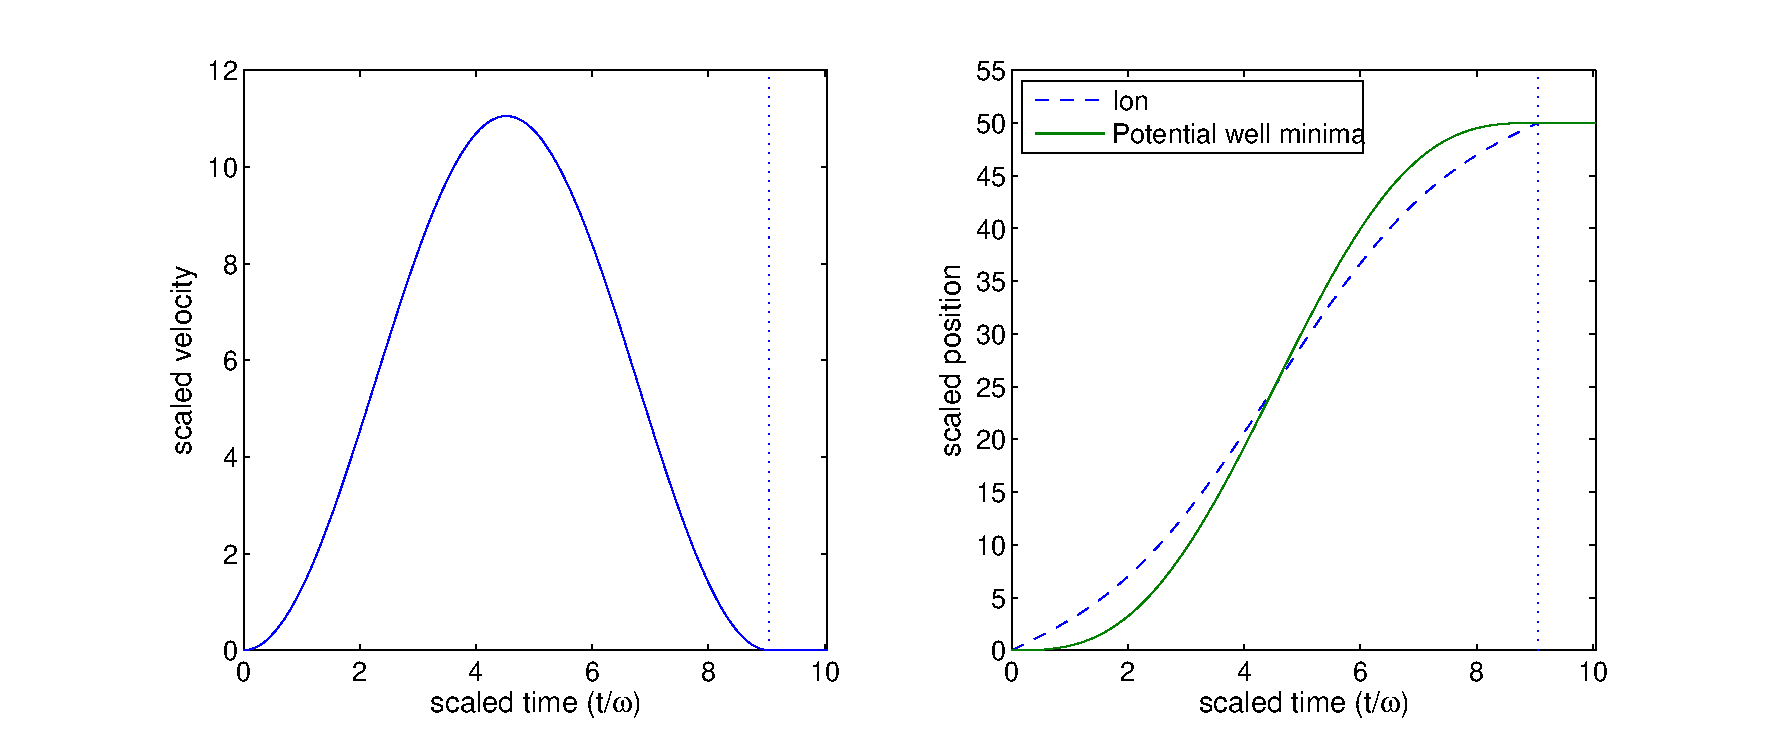
\includegraphics[width=15.5cm]{chapter3/movewell/movewell_example_combined_01}
% \caption[Theoretical single ion shuttle curve]{(Left) Desired ion velocity and (Right) corresponding ion position (solid line) and well position (dashed line) as functions of time, in scaled units. The vertical line denotes the end of the shuttle sequence.  }
% \label{fig:movewelleg}
% \end{figure} 

\begin{figure}[!t]
\begin{center}
$\begin{array}{cc}
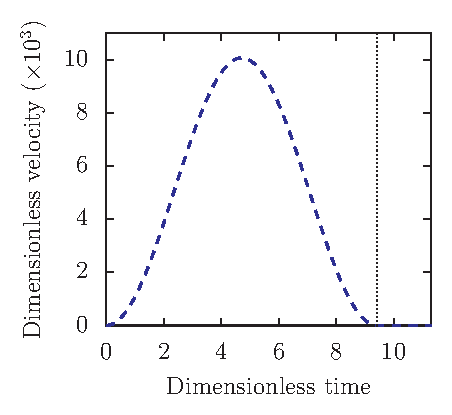
\includegraphics{chapter3/movewell/idealshuttle_t3_v} & 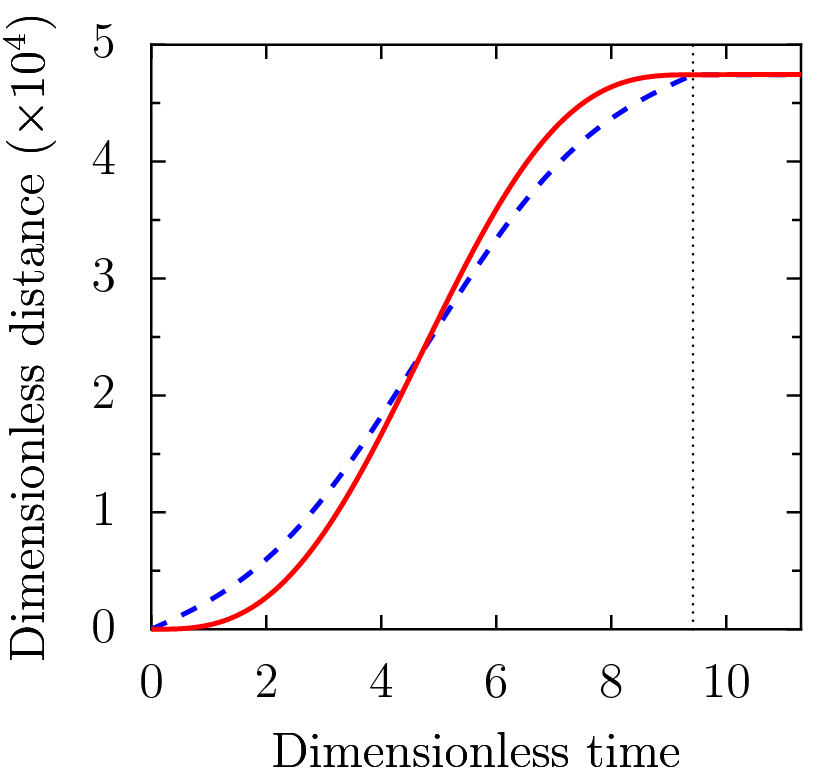
\includegraphics{chapter3/movewell/idealshuttle_t3} \\
\end{array}$
\end{center}
\caption[Theoretical single ion shuttle curve]{(Left) Desired ion velocity and (Right) corresponding ion position (solid line) and well position (dashed line) as functions of time, in scaled units. The vertical line denotes the end of the shuttle sequence. The shuttle distance is one electrode separation away from the trap centre (752.5\um). 
The time is expressed in units of $\omega^{-1}$, the distance in units of $\sqrt{\hbar / m \omega}$ and the velocity in units of $v_0 = \sqrt{\hbar \omega/m}$.
%Dimensionless units for time is $t_0 = \omega^{-1}$, for distance $x_0 = \sqrt{\hbar / m \omega}$ and for velocity $v_0 = \sqrt{\hbar \omega/m}$.
}
\label{fig:movewelleg}
\end{figure} 



Once $x_0(t)$ is available, it has to be turned into practical voltage sequences to control the ion trap electrodes. This can be done either by numerically simulating the ion trap's behaviour (as illustrated in the previous chapter), or by experimentally mapping control voltages onto trapping positions and frequencies. Figure~\ref{fig:theoryshuttle} shows a voltage control sequence to shuttle an ion from the centre of the Liverpool trap through one electrode distance (0.7525\mm), corresponding to the potential well control of Figure~\ref{fig:movewelleg}. Voltages on only two electrodes are shown; the other 5 electrodes are kept at a constant voltage. 

 \begin{figure}[h!t]
 \centering
% 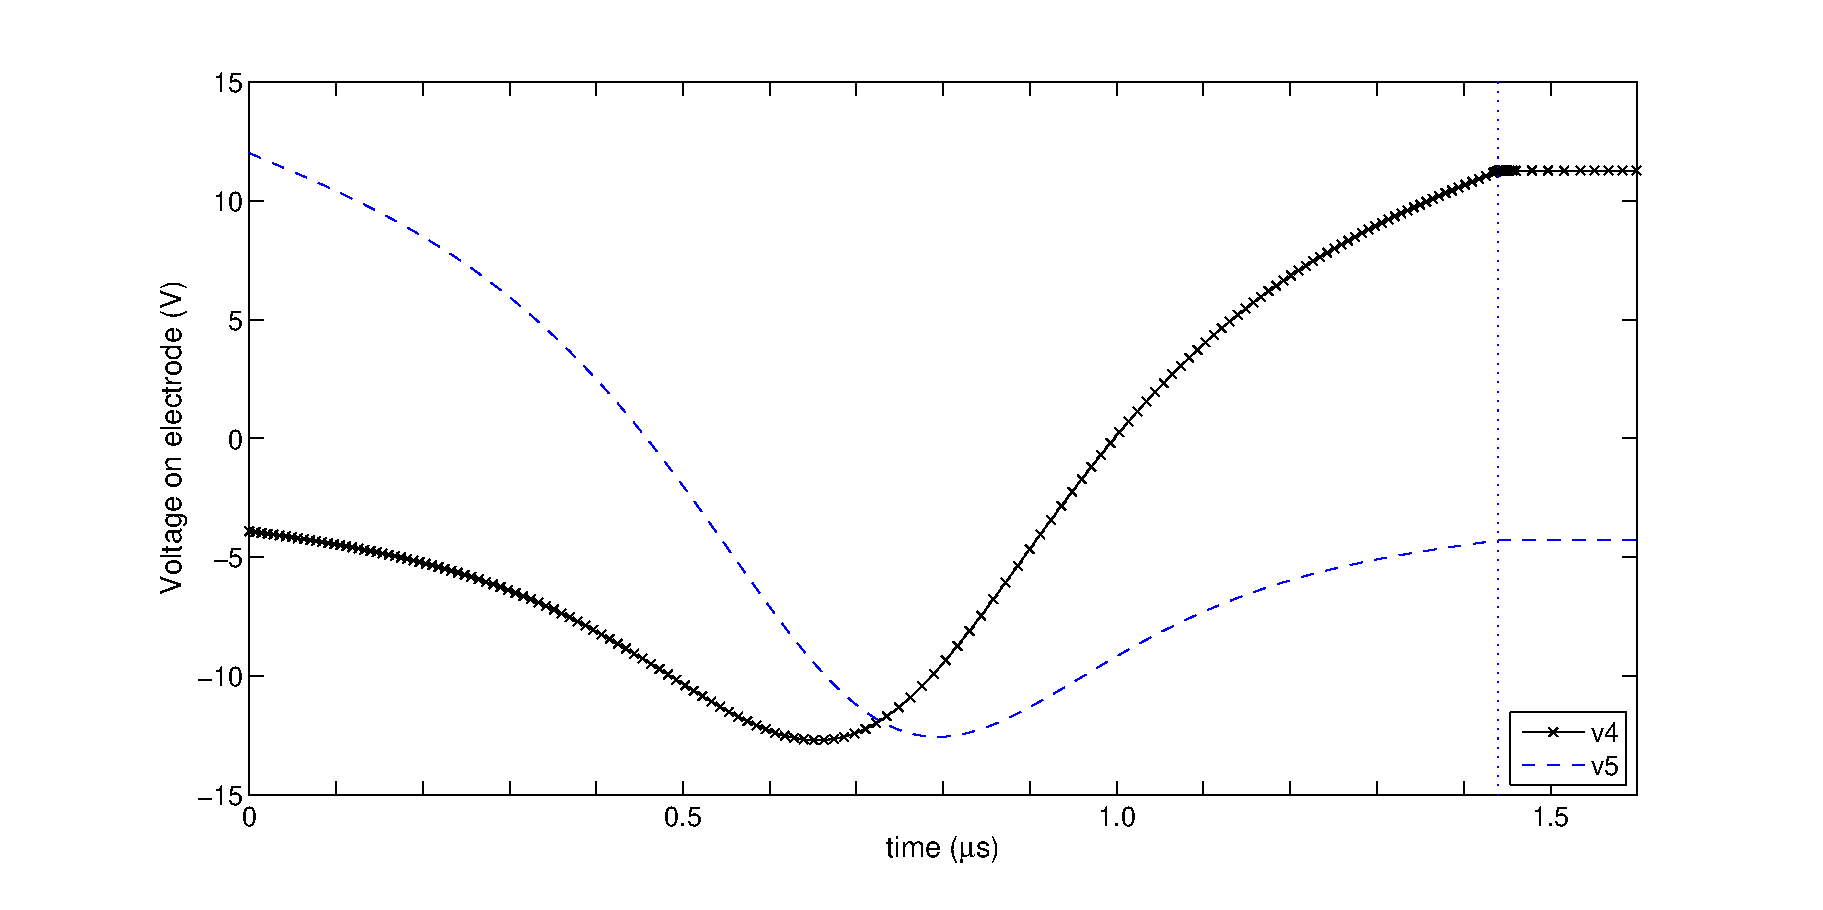
\includegraphics[width=15.5cm]{chapter3/movewell/shuttlevoltage_v01}
 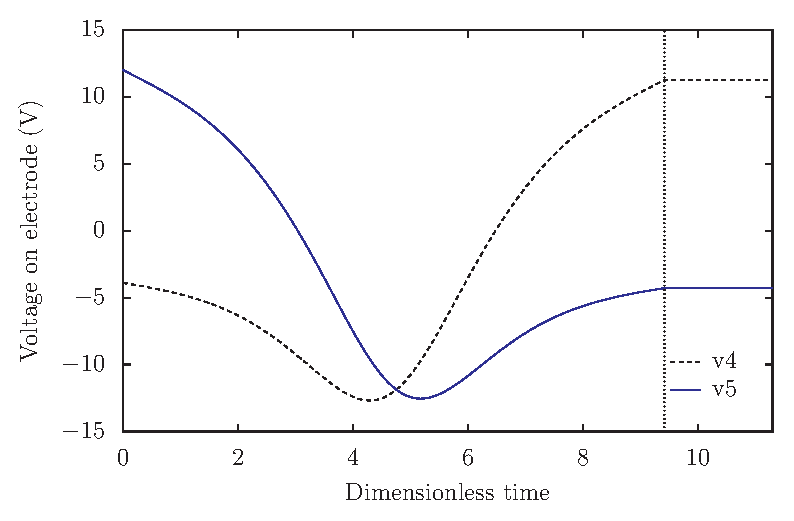
\includegraphics{chapter3/movewell/idealshuttle_t3_volts}
 \caption[Example voltage sequence for single ion shuttle]{Example shuttle voltage sequence in the Liverpool trap. The ion is moved by one electrode distance (0.755\mm) from in front of electrode \#4 to \#5, using the shuttle sequence shown in Figure~\ref{fig:movewelleg}. Voltages on electrode \#4 and \#5 are shown, while all other electrodes are kept at 12\V. The trap frequency is kept at $\omega/2\pi = 1\MHz$. A vertical line denotes the end of the shuttle sequence.}
 \label{fig:theoryshuttle}
 \end{figure} 


\begin{figure}[h!t]
\centering
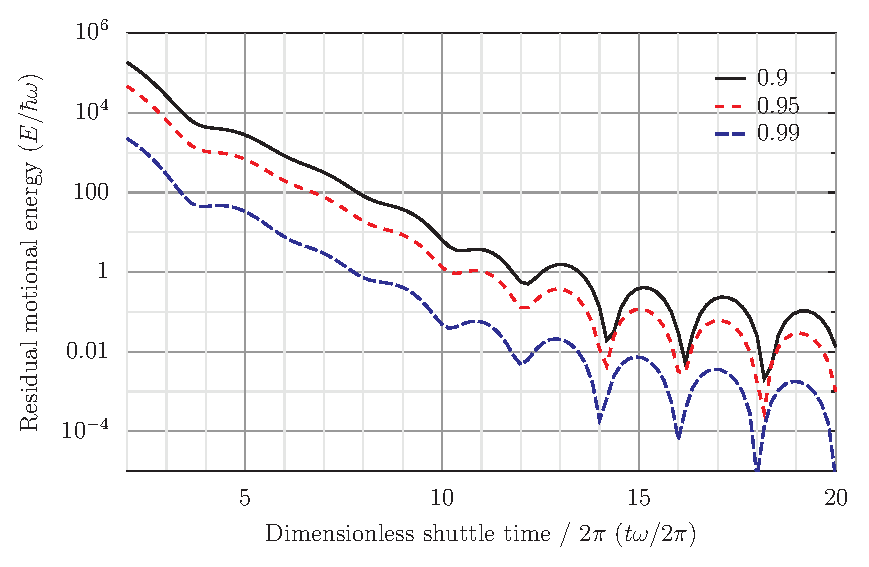
\includegraphics{chapter3/movewell/moveheat}
\caption[Heating due to imperfect shuttle voltages]{Excess heating as a function of total shuttle time, for different changes in control voltages compared to the expected voltages. Multipliers $\{0.90,0.95,0.99\}$ mean $\{10\%,5\%,1\%\}$ lower voltages than expected control voltage (see text). The ion is shuttled to one electrode distance, that is $x/\sqrt{\hbar/m w} = 4.7\times 10^4$ in dimensionless units. }
\label{fig:moveheat}
\end{figure} 


It is important to estimate the effect of control parameter imperfections on the outcome of the shuttle. There are a large number of error models and testing for all of them would not be practical. We present a calculation in case of a simple error model that can arise in experimental situations: imperfect setting of control voltages. In our calculation we assumed that compared to the voltages presented in Figure~\ref{fig:theoryshuttle}, the voltage of the centre electrode (v4) is changed by a fixed multiplier. Multipliers of $\{0.90,0.95,0.99\}$ are used. The change in trap frequency was 2.6\%-0.1\% along the shuttle path in case of the $0.9$ multiplier, and smaller for the other multipliers.

Figure~\ref{fig:moveheat} shows the ion's excess motional energy, as a function of shuttle time. The results show that even when the control voltage is 10\% different from the expected voltage, the ion can be shuttled by one electrode separation distance (752.5\um) in $t = 12 / (\omega/2\pi) = 12\us$ while gaining only a single motional quantum.


From an experimental point of view, however, fast changes in the voltages might pose challenges to the control electronics. The shuttling DC control voltages such as the one in Figure~\ref{fig:theoryshuttle} have complicated time dependence and must be generated with good timing and precision.
Also, in most of the ion trap designs the voltage supply lines of the DC electrodes have low-pass filters installed to reduce noise and heating of the ion. These filters will change the waveforms, and introduce Johnson noise heating into the ion transport. In this situation one should analyse the effect of the filters on the waveforms and change the input voltage control sequence to achieve the desired output after the filters. If this is not possible, then one has to perform slower ion shuttling. The filters may also be advantageous in case of using Digital-to-Analog converters to create the control voltages: the digitization effects can be blurred out by the filters, resulting in a better voltage sequence on the electrodes.

This method is also applicable to separating and joining ions. In the calculations the Coulomb interaction of the ions can be taken into account as a short distance perturbation of the trapping potential. Figure~\ref{fig:moveseparate} shows a voltage sequence and two ion trajectories in the case of separating two ions. To join them together requires simply the time-reversal of the applied voltages. 

 \begin{figure}[h!t]
\begin{center}
$\begin{array}{cc}
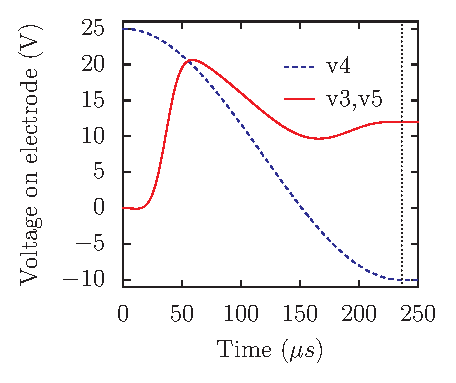
\includegraphics{chapter3/movewell/splitvolts_1} & 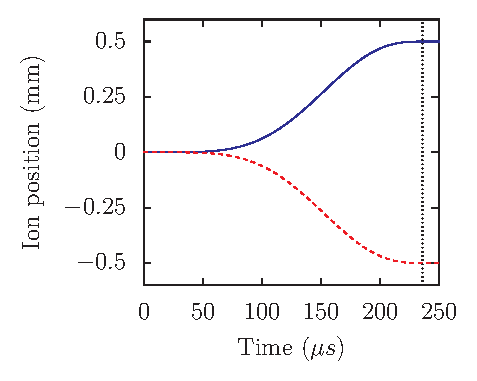
\includegraphics{chapter3/movewell/splitvolts_2_v2} \\
\end{array}$
\end{center}
 \caption[Example voltage sequence for ion separation]{(Left) Voltage sequence to perform ion separation. The voltage on electrode \#4 and those on \#3,\#5 (the same) are shown, all other electrodes are at 25\V. (Right) simulated ion trajectories during separation. The vertical dotted line marks the end of the shuttling sequence. The time scale is longer than on the previous plots, to provide a voltage control sequence that may be be experimentally produced (due to the limit on the rate of change of DC control voltage). The calculation can be carried out in a similar manner for faster separation. The maximum separation was 1\mm. The electrode-electrode distance is 0.7525\mm.}
 \label{fig:moveseparate}
 \end{figure} 

% \begin{figure}[h!t]
% \centering
% 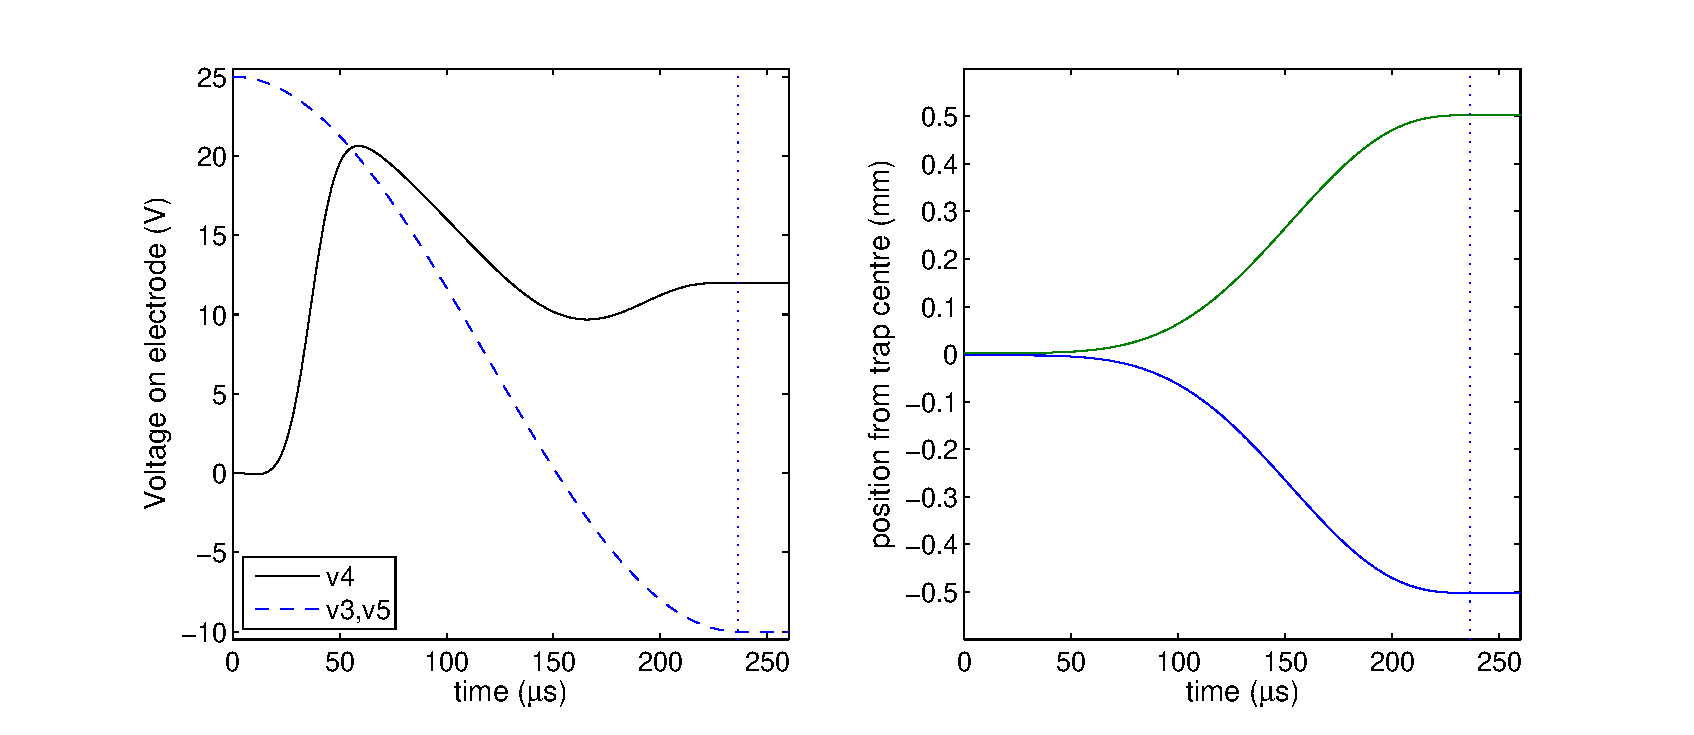
\includegraphics[width=15.5cm]{chapter3/movewell/moveseparate}
% \caption[Example voltage sequence for ion separation]{(Left) Voltage sequence to perform ion separation. The voltage on electrode \#4 and those on \#3,\#5 (the same) are shown, all other electrodes are at 25\V. (Right) simulated ion trajectories during separation. The vertical dotted line marks the end of the shuttling sequence. The time scale is longer than on the previous plots, to provide a voltage control sequence that may be be experimentally produced (due to the limit on the rate of change of DC control voltage). The calculation can be carried out in a similar manner for faster separation. The maximum separation was 1\mm. The electrode-electrode distance is 0.7525\mm.}
% \label{fig:moveseparate}
% \end{figure} 


Extending this approach to 2D movements, such as around a corner at a junction (as in \cite{Hensinger2006}), and the analysis of imperfections of timing and trap frequency require additional theoretical work and will be the subject of a later study.


\section{Ion loading simulation in Sandia trap}

After observing neutral \CaI{} fluorescence in the Sandia trap, trapping of ions was attempted. However, for a period of time, this was not successful. While exploring different experimental control parameters (photoionisation laser powers, Doppler-cooling laser powers and detunings, \CaI{} oven currents, etc.), the electrical parameters of the trap could not of course be measured directly. Before trapping ions, one has only limited means of evaluating what voltages are actually on the electrodes. In the case of the DC electrodes the uncertainty was mainly whether the applied voltage reaches the electrode, or there is an electrical break along the way. In the case of the RF electrodes the situation is more subtle. The drive voltage was amplified by a helical resonator (see Section~\ref{sec:helicalresonator}). The amplification (Q-value) was estimated, but losses could occur on the electrical connections bridging the outer and inner side of the vacuum can. Thus we had an upper estimate of voltages ($\sim 100\V$), and the actual RF amplitude could have taken any value up to this.

To evaluate the effect of different RF amplitudes on the ion loading rate, a numerical study was conducted. The electric field was modelled in the Sandia trap, as described in the previous chapter. The resulting potentials were then used to generate an oscillating electric field. An ion was randomly placed in the area near the the trap centre, where the photoionisation and Doppler-cooling laser beams were focused (with radii $\sim 20\um$). The random placement represented the ionization happening at that particular position, and the ion suddenly starting to interact with the RF field. The subsequent behaviour of the ion was found by solving the classical equation of motion. Table~\ref{tab:loadsimparams} lists the initial parameters. The ion's movement was followed for a number of RF cycles, to evaluate whether it had a trapped orbit or leaves the trap. Doppler cooling was not included in the simulation, since it is too slow to affect the results. If the RF field on its own would not trap the ion, the cooling would not in general prevent it from escaping. 


\begin{table}[ht]
 \begin{center}
% use packages: array
\begin{tabular}{|c|c|}
\hline
\textbf{Parameter} & \textbf{Values} \\ 
\hline
Starting position 			&  Random in area, $r < 20\um$ \\ 
Starting velocity 	& Random, 0-700\K (100\K steps)\\ 
Direction of velocity 	& Set, 45\degree to trap electrode plane \\
RF phase & Random \\
RF amplitude $V_{\rm rf}$ & 25,40,50,60,75,100\V \\
\hline
\end{tabular}
\end{center}
\caption{Ion loading simulation parameters}
\label{tab:loadsimparams}
\end{table}


Figure~\ref{fig:sampletraptrace} shows two sample ion trajectories. The trap electrodes lie in the X-Z plane and the RF electrodes are at $x=\pm100\um$. The direction of the initial velocity of the ion was set by the respective positions of the \CaI{} oven and the trap (see Figure~\ref{fig:angles}), that is, at 45\degree, from the bottom-left to the top-right in Figure~\ref{fig:sampletraptrace}.

Figure~\ref{fig:captureprobvolt} summarizes the overall capture probabilities as a function of ion temperatures (starting velocities), for different RF amplitudes. For RF amplitudes $V_{\rm rf} < 50\V$ the capture probability of high temperature ions is significantly reduced. Since the \CaI{} oven was expected to operate at temperatures $\sim 600\K$, a large fraction of the ions is expected to have even larger velocities than those considered in the simulation. Thus the requirement for successful trapping in the Sandia trap appears to be $V_{\rm rf} > 50\V$. 

Figure~\ref{fig:captureprobtemp} shows an additional detail of the simulated ion loading. The capture probabilities are plotted as functions of distance from the trap centre for different ion temperatures. That is $P(r) =$ the proportion of ions created withing a disc of radius $r$ that are captured. The RF amplitude was set to $V_{\rm rf} = 50\V$, the lower limit of practical trapping. It appears that lower temperature ions are more likely to be captured in the inner regions of the trapping area, while the high temperature ions are captured in the outer regions. Figure~\ref{fig:captureposition} shows the initial positions of successfully trapped ions for $V_{\rm rf} = 50\V$ and $T = 500\K$. It appears that there is virtually no capture of ions which cross the trap centre. On the two sides of this central band ions are captured when the phase of the RF field is such that it deflects the ions towards the trap centre, and eventually they end up in a stable orbit. Correspondingly, the initial RF phase for the ions captured in the two areas are opposite to each other. 

Once ion loading was successful in the Sandia trap, and experiments were carried out to test the trap frequencies (see in Section~\ref{sec:ticleexperiment}), it was possible to relate the RF input voltages to the RF amplitude on the electrodes. It was found that the trap operation was in the $63\V<V_{\rm rf}<105\V$ region. This suggests that the difficulty of ion loading was due to other factors, while the electrical properties of the Sandia trap were adequate (see Section~\ref{sec:ionload}).


 \begin{figure}[h!t]
 \centering
 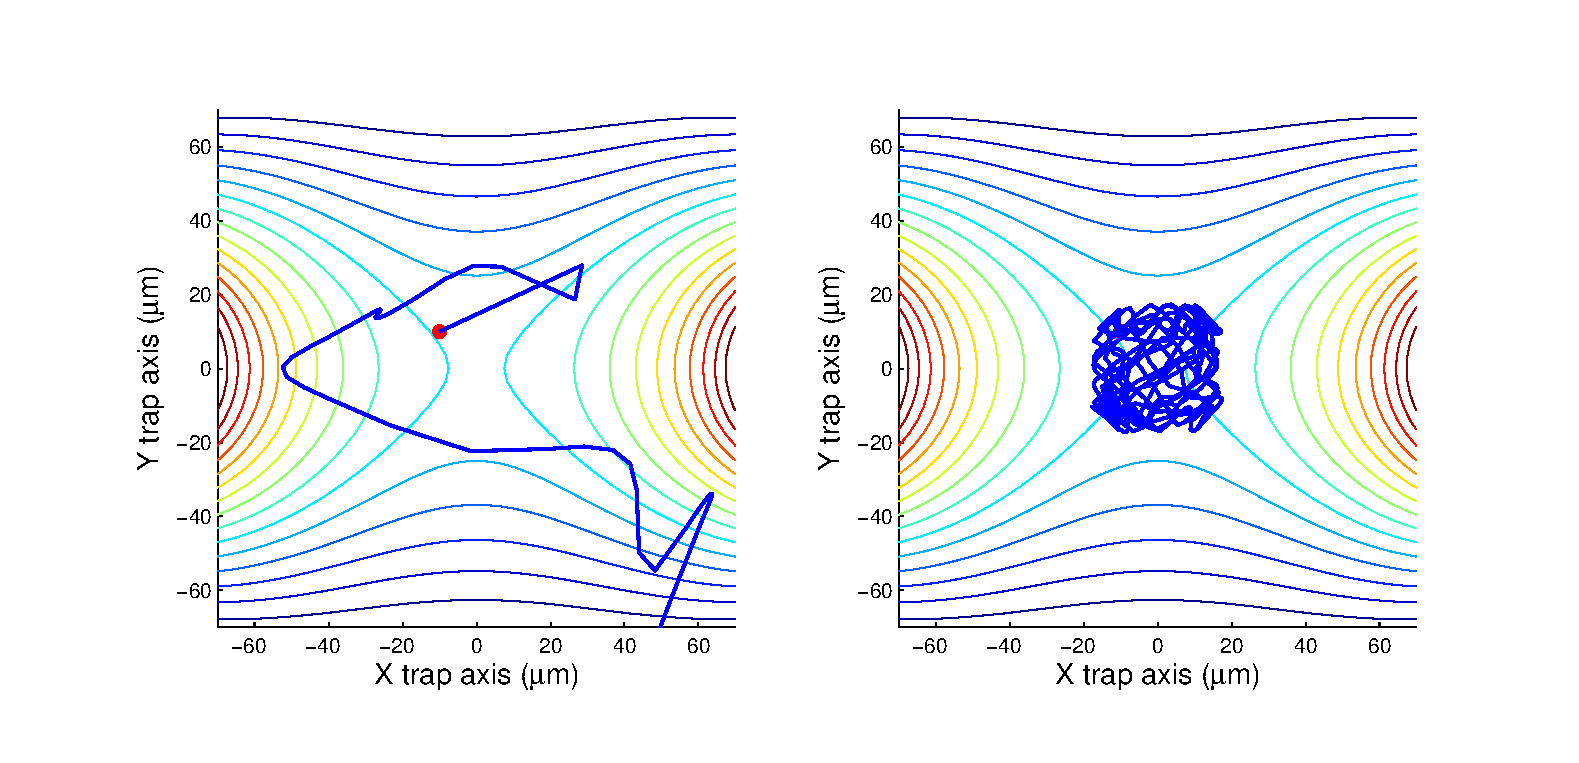
\includegraphics[width=14.5cm]{chapter3/tempcapture/motion_combined_v3}
 \caption[Trapped and non-trapped ion trajectories in Sandia trap]{Examples of simulated ion motion inside the trap. The trap electrodes lie in the X-Z plane; the static field lines are plotted for reference. The ion's initial position is indicated by a dot at the beginning of the trace, with velocity in the top-right direction. Both traces start at the same position and velocity, but at different points in the RF cycle (they have $\pi/2$ different phase). $V_{\rm rf} = 100\V$, $T_{ion} = 700\K$. The equation of the motion was solved with a variable step size Runge-Kutta method.}
 \label{fig:sampletraptrace}
 \end{figure} 


 \begin{figure}[h!t]
 \centering
% 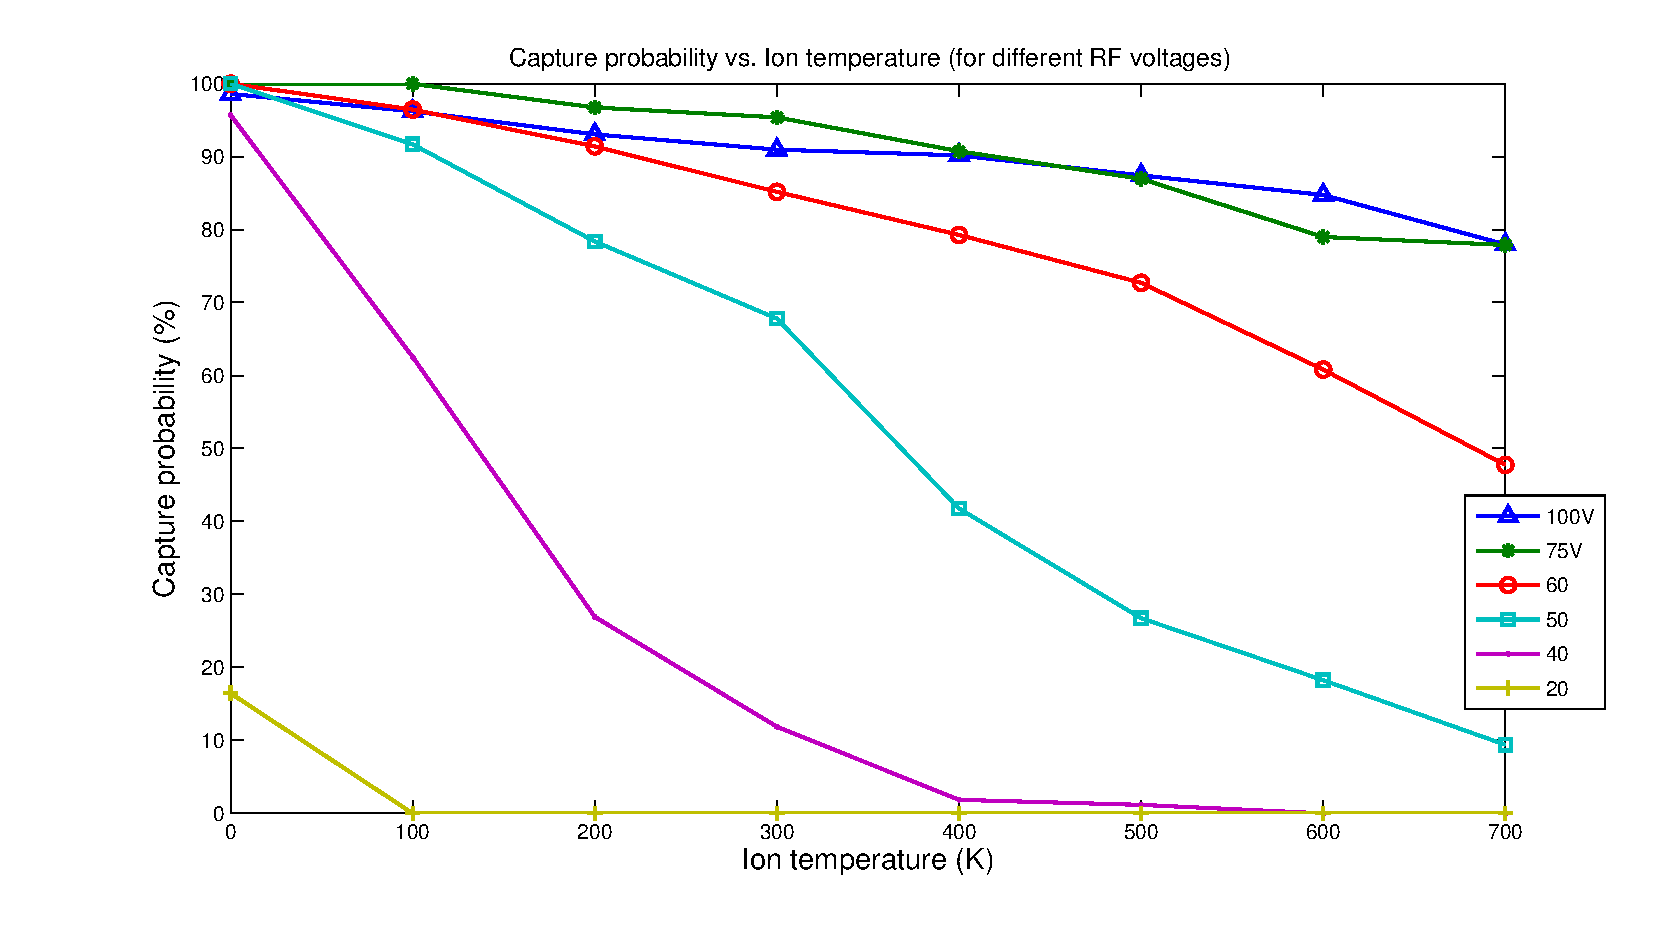
\includegraphics[width=14.5cm]{chapter3/tempcapture/temp_capture3}
% \caption[Ion capture probabilities in Sandia trap]{Summary of the overall capture probabilities within a 20\um\, radius of the trap centre, as a function of ion temperature, for different RF amplitudes.}
 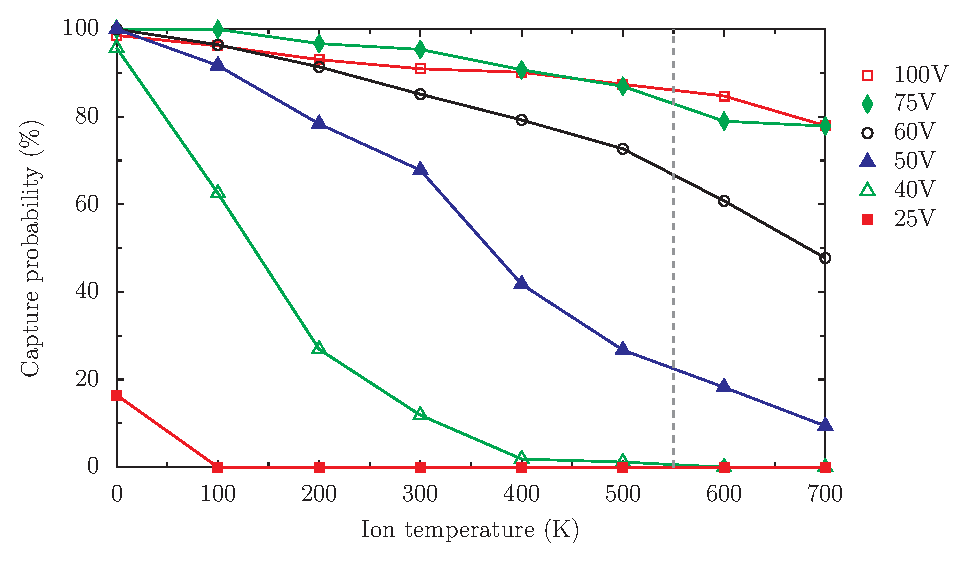
\includegraphics[width=14.5cm]{chapter3/tempcapture/temp_capture_v4}
 \caption[Ion capture probabilities in Sandia trap]{Summary of the simulated overall capture probabilities within a 20\um\, radius of the trap centre, as a function of ion temperature and RF amplitudes. Each point represents a single value of the initial ion speed $v$ and `ion temperature' is $m v^2 / \kB$. The dashed line shows the nominal \CaI{} oven temperature. Each data point is based on 700-3000 simulated ionisation events.}
 \label{fig:captureprobvolt}
 \end{figure} 


 \begin{figure}[h!t]
 \centering
 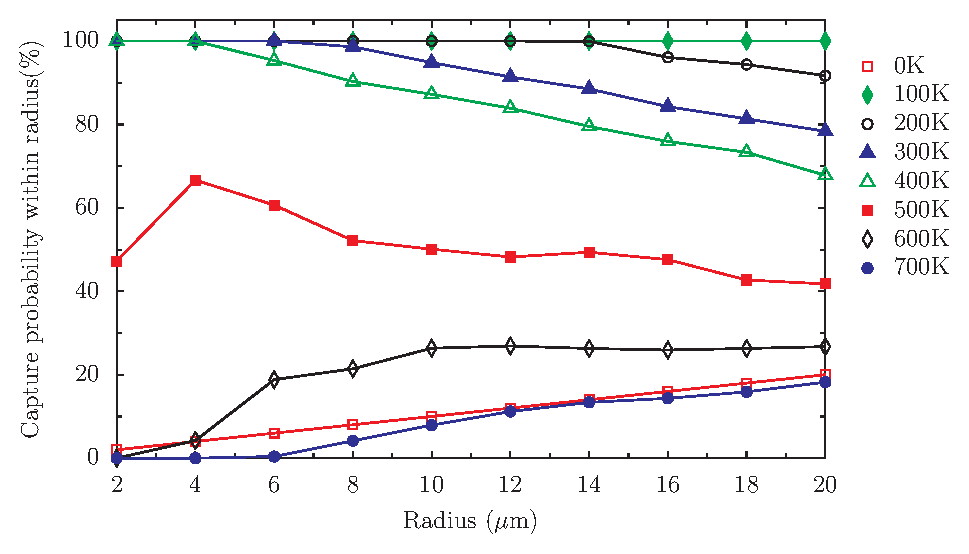
\includegraphics[width=13.5cm]{chapter3/tempcapture/capture_prob_50_v2}
 \caption[Capture probability as function of ionization position]{
Proportion of ions P(r), captured with ionisation position within radius $r$ from the trap centre, for a number of ion temperatures. The RF amplitude is set to $V_{\rm rf} = 50\V$.  Cold ions are more likely to be captured in the trap centre, while hot ions are more likely to be captured in the outer regions. The average density of simulated ionisation positions was 2.5 ion/$\um^2$ within the maximum 20\um\, radius.
%Capture-probabilities of ions P(r), as a function of the distance of their initial position from the trap centre, for different ion temperatures, and $V_{\rm rf} = 50\V$.  Cold ions are more likely to be captured in the trap centre, while hot ions are more likely to be captured in the outer regions. 
}
 \label{fig:captureprobtemp}
 \end{figure} 

% \begin{figure}[h!t]
% \centering
% 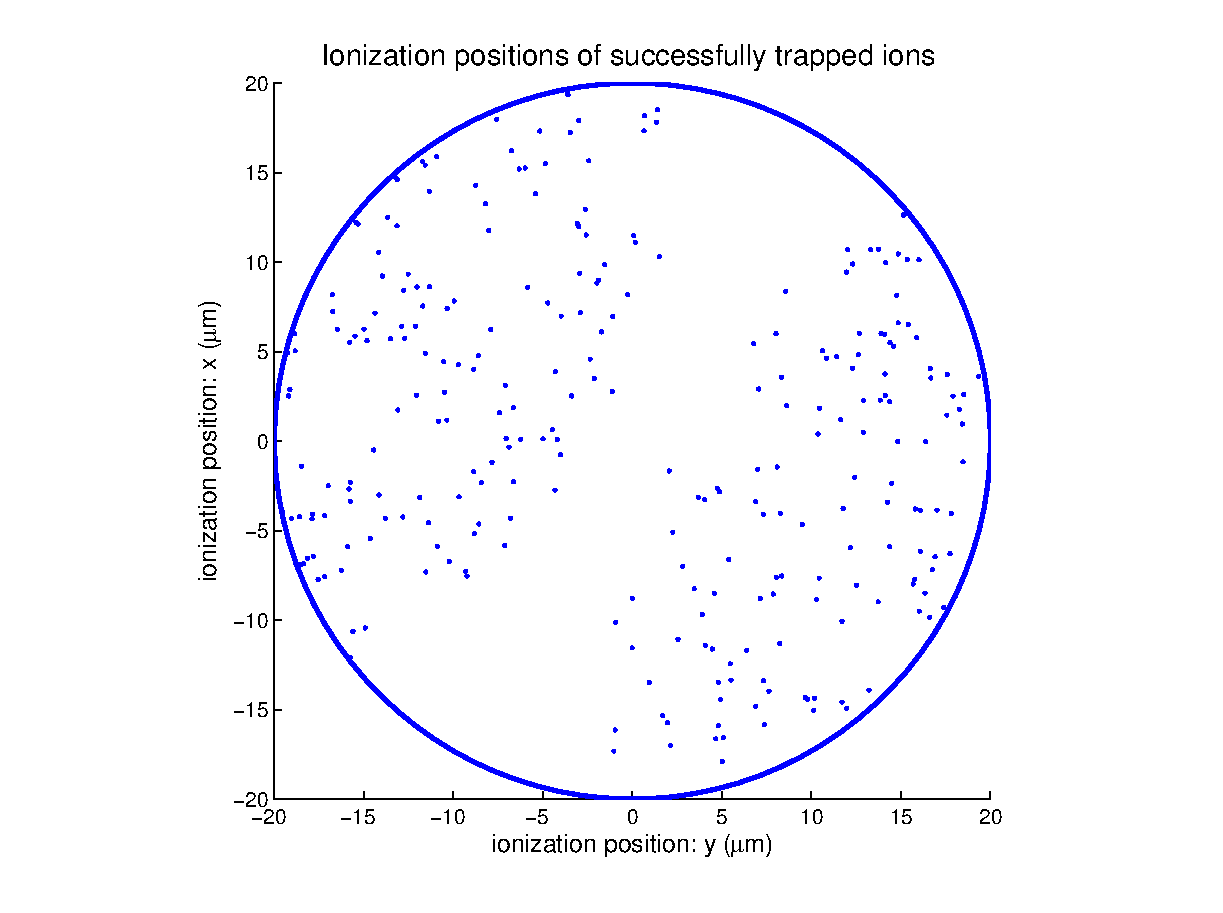
\includegraphics[width=12.5cm]{chapter3/tempcapture/ipos_50_500_v2}
% \caption[Ionization positions of successfully trapped ions]{A number of ionization positions of successfully captured ions in the case of $V_{\rm rf} = 50\V$ and $T_{ion} = 500\K$. The ions' initial position is randomly distributed within the 20\um\, radius shown. The ions' initial velocity is in the (1,1) direction. The captured ions in the top left and the bottom right quadrant require opposite initial RF phase to be captured.}
% \label{fig:captureposition}
% \end{figure} 

 \begin{figure}[h!t]
 \centering
% 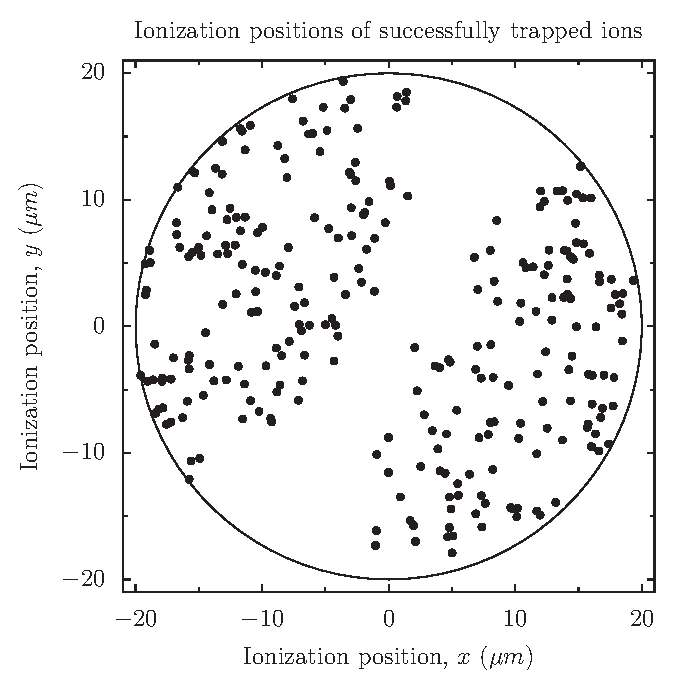
\includegraphics{chapter3/tempcapture/ionpos}
 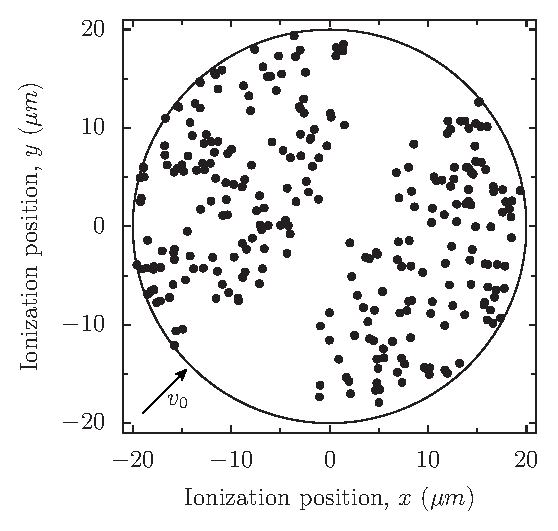
\includegraphics{chapter3/tempcapture/ionpos_v2}
 \caption[Ionization positions of successfully trapped ions]{A number of simulated ionization positions of successfully captured ions in the case of $V_{\rm rf} = 50\V$ and $T_{ion} = 500\K$. The ions' initial positions are randomly distributed in area within the 20\um\, radius shown. The direction of the ions' initial velocities is indicated by an arrow. The captured ions in the top left and the bottom right quadrant require opposite initial RF phase to be captured.}
 \label{fig:captureposition}
 \end{figure} 

